\subsection{Contexto da Pesquisa} \label{subsec:contexto}
%Torna a análise de séries temporais e previsões valiosas ferramentas para apoiar o processo de tomada de decisão a curto, médio e longo prazo. Devido às não linearidades, sazonalidade, tendência e que podem ocorrer em séries temporais de abastimento de água nos dados temporais, o desenvolvimento de modelos de previsão eficientes é uma tarefa desafiadora \cite{mateus}.
%
%Na Figura \ref{fig:paradigma-ml}, são mostradas as etapas de como deve ocorrer a análise de dados e a seleção dos modelos. Essa seleção pode ser feita de forma que se tenha que escolher o que deve ser previsto na variável. Feito isso, temos a primeira etapa que será dos dados, depois que cada um foi identificado com seus rótulos de entrada e saída. Os dados não podem conter \textbf{NaN} (do inglês \textit{not a number}) ou dados ausentes, o que evita falsos positivos. 

Torna-se evidente que a análise de séries temporais e previsões são ferramentas valiosas para apoiar o processo de tomada de decisão em curto, médio e longo prazo. Devido às não linearidades, sazonalidades e tendências que podem ocorrer nos dados temporais de abastecimento de água, o desenvolvimento de modelos de previsão eficientes torna-se uma tarefa desafiadora \cite{mateus}.

Na Figura \ref{fig:paradigma-ml}, as etapas de como a análise de dados e a seleção dos modelos devem ocorrer são apresentadas. Essa escolha pode ser conduzida de modo a determinar o que deve ser previsto na variável. Feito isso, a primeira etapa envolve a preparação dos dados, garantindo que cada um tenha sido identificado com seus rótulos de entrada e saída. É imperativo que os dados não contenham \textbf{NaN} (do inglês \textit{not a number}) ou dados ausentes, evitando assim falsos positivos.

\begin{figure}[!htb]
	\centering
	\caption{Paradigma de aprendizado de máquina}
	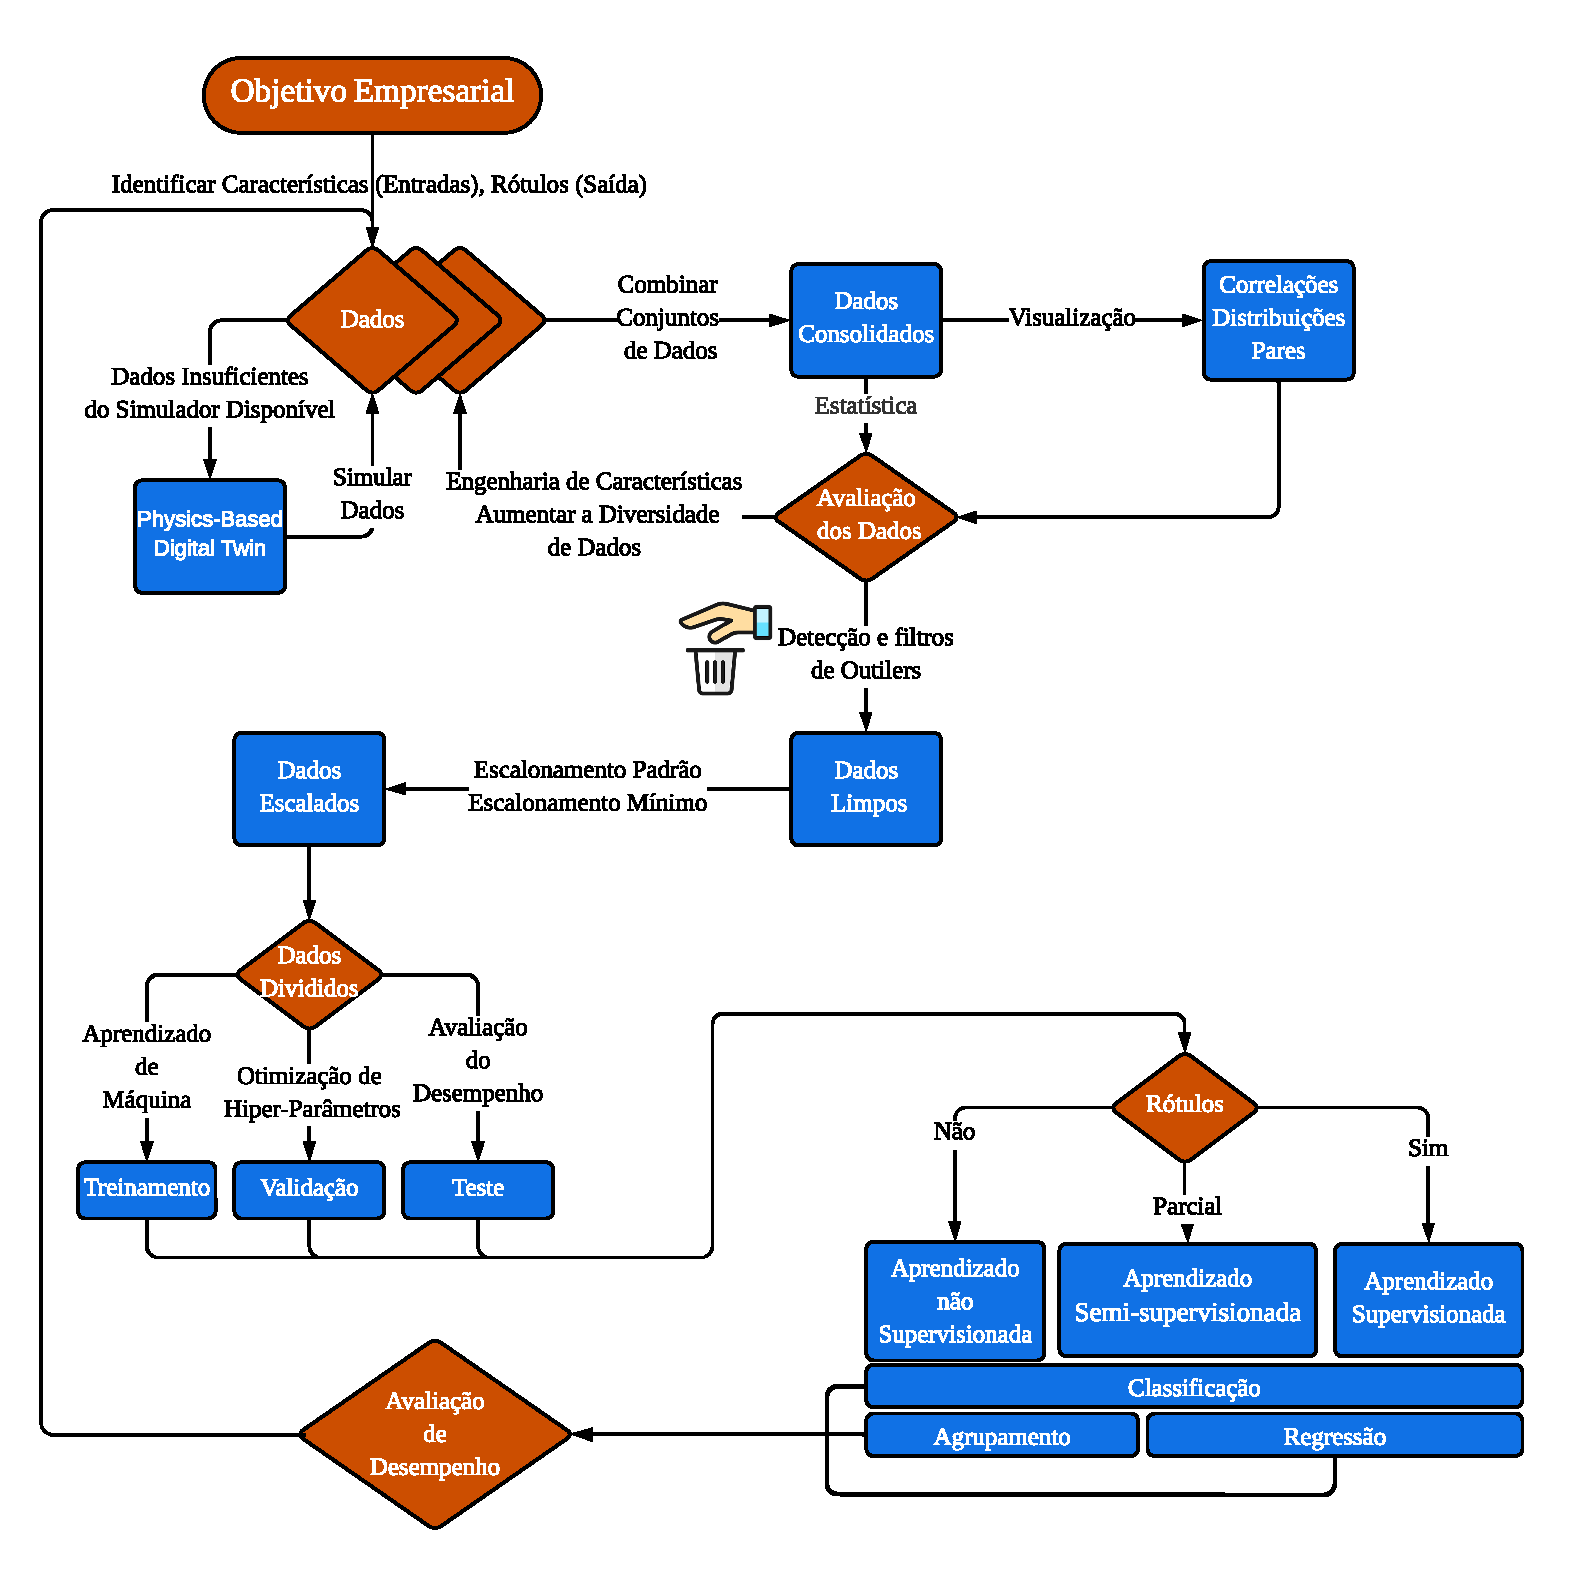
\includegraphics[width=\linewidth]{Introducao/Figuras/paradigma-ml}
	
	\fonte{Adaptado de \cite{apmonitor}}
	\label{fig:paradigma-ml}
\end{figure}

Ao realizar essa etapa, a pessoa deve visualizar os dados para garantir que estejam carregados corretamente e em um tamanho tolerável, o que é conhecido como avaliação dos dados. Uma vez que os dados estejam limpos e devidamente carregados, sem falsos positivos, a divisão dos dados pode ser efetuada.
A otimização dos dados para os modelos pode ocorrer de diversas maneiras, como a utilização da biblioteca Optuna em Python, que emprega a otimização Bayesiana para cada modelo pré-listado, reduzindo assim o tempo de processamento.

A validação é uma prática comum em conjuntos de dados extensos, permitindo que os modelos interajam mais eficientemente com os dados e proporcionem resultados mais precisos. Após essa etapa, na escolha dos modelos, há a possibilidade de determinar se o modelo é de série temporal, classificação, agrupamento ou regressão. Posteriormente, ao listar os modelos, cada um deles deve passar por uma avaliação com métricas específicas para verificar a precisão de seus resultados.

%Fazendo isso, os dados podem ser visualizados para garantir que estejam bem carregados e que estejam em um tamanho tolerável. Isso é chamado de avaliação dos dados. Com os dados limpos e bem carregados, sem falsos positivos, a divisão dos dados pode ser feita. 
%
%A otimização dos dados para os modelos pode ser realizada de várias formas, como o uso da biblioteca do python Optuna que usa otimização Bayesiana para cada modelo pré-listado, reduzindo assim o tempo de processamento. 
%
%A validação é comum em conjuntos de dados muito grandes para permitir que os modelos trabalhem mais com os dados, proporcionando resultados mais precisos. Após essa etapa, na escolha dos modelos, há a possibilidade de escolher o modelo de série temporal, se o modelo é de classificação, agrupamento ou regressão. Após listar os modelos, cada um deles deve ser avaliado em métricas para verificar a veracidade de cada um.



  
      
\subsubsection{Motiva\c c\~ao da Pesquisa} \label{subsubsec:motivacao}

A motivação desta pesquisa baseia-se na situação enfrentada por Curitiba e região metropolitana, conforme destacado por \cite{vasconcelos_2020}. A região passou por um rodízio de abastecimento de água, com períodos de 36 horas com abastecimento de água, seguidos por 36 horas sem abastecimento. A média geral dos reservatórios na região estava em torno de $27,96\%$ de sua capacidade. Além disso, a quantidade de chuva nos anos anteriores, em $2020$, foi de $1.704$ mm, superando a média anual de precipitação de $1.490$ mm.

Diante dessa situação, a pesquisa tem como abordagem principal a previsão do abastecimento de água, associada a condições de seca ou decorrentes das consequências da COVID-19. A partir dos dados coletados pela SANEPAR, é possível realizar uma análise detalhada, com o objetivo de prever e evitar a ocorrência de escassez de água. 
 
%A motivação desta pesquisa é baseada na situação enfrentada por Curitiba e região metropolitana, conforme apontado por \cite{vasconcelos_2020}. A região passou por um rodízio de abastecimento de água, com períodos de 36 horas com abastecimento de água seguidos por 36 horas sem abastecimento de água. A média geral dos reservatórios na região estava em torno de $27,96\%$ de sua capacidade. Além disso, a quantidade de chuva nos anos anteriores, de $2020$, foi de $1.704$ mm, superando a média anual de precipitação de $1.490$ mm.
% 	
%Diante dessa situação, a pesquisa tem como abordagem principal a previsão do abastecimento de água, que pode ser associada a condições de seca ou decorrentes das consequência da COVID-19. A partir dos dados coletados pela SANEPAR, é possível realizar uma análise detalhada, com o objetivo de prever e evitar a ocorrência de escassez de água. 
%    
     
    